\documentclass[border=0.2cm]{standalone}
 
% Required Package and Librarie
\usepackage{pgfplots}
\usepackage{tikz}
\pgfplotsset{compat=newest}
\usepgfplotslibrary{fillbetween}
 
\begin{document}

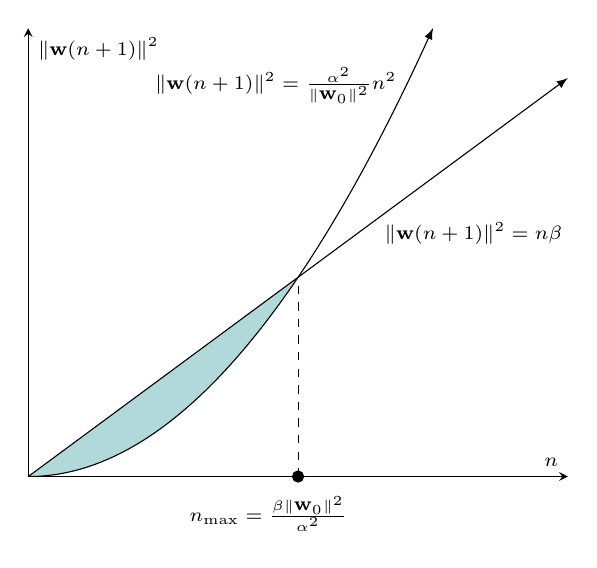
\begin{tikzpicture}
  \begin{axis}[
      axis lines = middle,
      xlabel = {\scriptsize $n$},
      ylabel = {\scriptsize $\Vert\textbf{w}(n+1)\Vert^2$},
      ticks = none
      % xmin=0, xmax=5.5,
      % ymin=0, ymax=24,
      % xtick={-3,-2,...,3}, ytick={-3,-2,...,3}
      ]

    % Plot 1
    \addplot [name path = A,
      -latex,
      domain = 0:3,
      samples = 1000] {2*x^2}
    node [very near end, left] {\scriptsize $\Vert\textbf{w}(n+1)\Vert^2=\frac{\alpha^2}{\Vert\textbf{w}_0\Vert^2}n^2$};

    % Plot 2
    \addplot [name path = B,
      -latex,
      domain = 0:4] {4*x}
    node [pos=1, below] {};
    \addplot[mark=*] coordinates {(2,0)};
    % Fill area between paths
    \addplot [teal!30] fill between [of = A and B, soft clip={domain=0:2}];
    \draw [dashed] (axis cs:{2,0}) -- (axis cs:{2,8});

    \node [label=below:{\scriptsize $\Vert\textbf{w}(n+1)\Vert^2=n\beta$}] (nmax) at (3.3, 11) {};

  \end{axis}
  \node [label=below:{\scriptsize$n_{\rm max}=\frac{\beta\Vert\textbf{w}_0\Vert^2}{\alpha^2}$}] (nmax) at (3.05, 0) {};
\end{tikzpicture}

\end{document}